% !TEX program = latexmk
% !TEX options = -xelatex --shell-escape -synctex=1 -interaction=nonstopmode -halt-on-error -file-line-error -f "%DOC%"
% Timeline with support windows and EOL years (past + active)

\documentclass[preview,tikz,dvipsnames, border=12pt,convert={density=600, png}]{standalone}

\usepackage{bold-extra}
\usepackage{amssymb,amsfonts,amsmath}
\usepackage{bm}
\newcommand{\vect}[1]{\mathbf{#1}}

\definecolor{UbuntuOrange}{HTML}{E95420}
\definecolor{UbuntuPurple}{HTML}{77216F}
\definecolor{ROSBlue}{HTML}{22314E}
\definecolor{GazeboOrange}{HTML}{F58113}
\definecolor{GazeboWhite}{HTML}{FFFFFF}
\definecolor{IgnitionLightOrange}{HTML}{E5B533}
\definecolor{IgnitionDarkOrange}{HTML}{DE6921}
\definecolor{EolGray}{HTML}{9A9A9A}

\usepackage{graphicx}
\usetikzlibrary{quotes,angles,calc,shapes,arrows.meta,positioning, decorations.markings, backgrounds}

\tikzset{
  event/.style = {circle, fill, minimum size=1, line width=.1pt},
  timeline/.style = {draw, thick,  shorten <=10pt,shorten >=10pt},
  arrow/.style={thick, ->},
  line/.style={thick, -},
  white background/.style={
        show background rectangle,
        tight background,
        background rectangle/.style={
            fill=white
        }
    },
}

\def\yUbuntu{-1.2}
\def\yRos{-3.5}
\def\yRosTwo{-5.8}
\def\yGazebo{-8.3}
\def\yIgnition{-10.5}

% Reference date for active vs past styling
\pgfmathsetmacro{\todayY}{2026.5}

% Support / EOL under the release line:
%   #1 color  #2 row y  #3 release year  #4 EOL year  #5 slot (0,1,2,...)
\newcommand{\supportbar}[5]{%
  \pgfmathsetmacro\xstart{2*(#3-2016)}%
  \pgfmathsetmacro\xend{2*(#4-2016)}%
  \pgfmathsetmacro\ybar{#2 - 0.30 - 0.14*#5}%
  \pgfmathtruncatemacro\eoly{floor(#4)}%
  \pgfmathtruncatemacro\isPast{ifthenelse(#4<\todayY,1,0)}%
  \ifnum\isPast=1
    \draw[EolGray, opacity=0.22, thin]
      (\xstart, #2-0.10) -- (\xstart, \ybar);%
    \fill[EolGray, opacity=0.28, rounded corners=0.5pt]
      (\xstart, \ybar-0.045) rectangle (\xend, \ybar+0.045);%
    \draw[EolGray, opacity=0.75, line width=0.7pt]
      (\xend, \ybar-0.11) -- (\xend, \ybar+0.11);%
    \node[anchor=west, inner sep=1.5pt, font=\scriptsize\ttfamily, text=EolGray]
      at (\xend, \ybar) {\eoly};%
  \else
    \draw[#1, opacity=0.28, thin]
      (\xstart, #2-0.10) -- (\xstart, \ybar);%
    \fill[#1, opacity=0.48, rounded corners=0.6pt]
      (\xstart, \ybar-0.055) rectangle (\xend, \ybar+0.055);%
    \draw[#1, line width=1.0pt]
      (\xend, \ybar-0.13) -- (\xend, \ybar+0.13);%
    \node[anchor=west, inner sep=1.5pt, font=\scriptsize\ttfamily, text=#1]
      at (\xend, \ybar) {\eoly};%
  \fi
}

\newcommand{\distrubuntu}[2]{% name, year
  \pgfmathsetmacro\x{2*(#2-2016)};
  \node[event=1.5pt, shading=axis, left color=UbuntuPurple, right color = UbuntuOrange, shading angle=135] (#1) at (\x,\yUbuntu){};
  \node[above=0.08 of #1, fill=white, inner sep=1pt]{\textcolor{UbuntuPurple}{\texttt{#1}}};
}

\newcommand{\distrros}[2]{% name, year
  \pgfmathsetmacro\x{2*(#2-2016)};
  \node[event=1.5pt, fill=ROSBlue] (#1) at (\x,\yRos){};
  \node[above=0.08 of #1, fill=white, inner sep=1pt]{\textcolor{ROSBlue}{\texttt{#1}}};
}

\newcommand{\distrrostwo}[2]{% name, year
  \pgfmathsetmacro\x{2*(#2-2016)};
  \node[event=1.5pt, fill=ROSBlue] (#1) at (\x,\yRosTwo){};
  \node[above=0.08 of #1, fill=white, inner sep=1pt]{\textcolor{ROSBlue}{\texttt{#1}}};
}

\newcommand{\gazeboversion}[2]{% name, year
  \pgfmathsetmacro\x{2*(#2-2016)};
  \node[event=1.5pt, shading=axis, left color=GazeboOrange, right color=GazeboWhite, shading angle=10] (Gazebo#2) at (\x,\yGazebo){};
  \node[above=0.08 of Gazebo#2, fill=white, inner sep=1pt]{\textbf{#1}};
}

\newcommand{\ignitionversion}[2]{% name, year
  \pgfmathsetmacro\x{2*(#2-2016)};
  \node[event=1.5pt, shading=axis, left color=IgnitionLightOrange, right color=IgnitionDarkOrange, shading angle=45] (Ignition#2) at (\x,\yIgnition){};
  \node[above=0.08 of Ignition#2, fill=white, inner sep=1pt]{\textbf{#1}};
}

\newcommand{\rosdistro}[1]{\textcolor{ROSBlue}{\texttt{#1}}}

\def\figScale{1}
\def\xLogo{-2}

\begin{document}

\begin{tikzpicture}[
    scale=\figScale,
    white background,
  ]
  \node(year) at (\xLogo, 0) {\textbf{Year}};
  \foreach \x in {0,2,...,30} {
    \pgfmathtruncatemacro{\year}{\x/2+2016}
    \node (\year) at (\x,0) {\textbf{\year}};
  }

  % --- Support windows (past = gray, active = color) ---
  % Ubuntu LTS
  \supportbar{UbuntuPurple}{\yUbuntu}{2016}{2021}{0} % xenial
  \supportbar{UbuntuPurple}{\yUbuntu}{2018}{2023}{1} % bionic
  \supportbar{UbuntuPurple}{\yUbuntu}{2020}{2025}{2} % focal
  \supportbar{UbuntuPurple}{\yUbuntu}{2022}{2027}{3} % jammy
  \supportbar{UbuntuPurple}{\yUbuntu}{2024}{2029}{4} % noble
  \supportbar{UbuntuPurple}{\yUbuntu}{2026}{2031}{5} % resolute

  % ROS 1
  \supportbar{ROSBlue}{\yRos}{2016}{2021}{0} % kinetic
  \supportbar{ROSBlue}{\yRos}{2017}{2019}{1} % lunar
  \supportbar{ROSBlue}{\yRos}{2018}{2023}{2} % melodic
  \supportbar{ROSBlue}{\yRos}{2020}{2025}{3} % noetic

  % ROS 2
  \supportbar{ROSBlue}{\yRosTwo}{2018}{2019}{0} % ardent–crystal
  \supportbar{ROSBlue}{\yRosTwo}{2019}{2021}{1} % dashing–eloquent
  \supportbar{ROSBlue}{\yRosTwo}{2020}{2023}{2} % foxy
  \supportbar{ROSBlue}{\yRosTwo}{2021}{2022}{3} % galactic
  \supportbar{ROSBlue}{\yRosTwo}{2022}{2027}{4} % humble LTS
  \supportbar{ROSBlue}{\yRosTwo}{2023}{2024}{5} % iron
  \supportbar{ROSBlue}{\yRosTwo}{2024}{2029}{6} % jazzy LTS
  \supportbar{ROSBlue}{\yRosTwo}{2025}{2026.9}{7} % kilted
  \supportbar{ROSBlue}{\yRosTwo}{2026}{2031}{8} % lyrical LTS

  % Gazebo Classic
  \supportbar{GazeboOrange}{\yGazebo}{2016}{2023}{0}

  % Gazebo / Ignition
  \supportbar{IgnitionDarkOrange}{\yIgnition}{2020}{2024}{0} % citadel
  \supportbar{IgnitionDarkOrange}{\yIgnition}{2021}{2022}{1} % edifice
  \supportbar{IgnitionDarkOrange}{\yIgnition}{2022}{2027}{2} % fortress LTS
  \supportbar{IgnitionDarkOrange}{\yIgnition}{2024}{2029}{3} % harmonic LTS
  \supportbar{IgnitionDarkOrange}{\yIgnition}{2025}{2026.9}{4} % ionic
  \supportbar{IgnitionDarkOrange}{\yIgnition}{2026}{2031}{5} % jetty LTS

  % Legend
  \node[anchor=west, font=\scriptsize, align=left, text=black!60] at (0, -12.1) {%
    \tikz\fill[ROSBlue, opacity=0.48, rounded corners=0.5pt] (0,0) rectangle (0.55,0.12);
    ~active support
    \quad
    \tikz\fill[EolGray, opacity=0.28, rounded corners=0.5pt] (0,0) rectangle (0.55,0.12);
    ~past support
    \quad
    \tikz\draw[ROSBlue, line width=0.9pt] (0,-0.08) -- (0,0.08);
    ~EOL year
  };

  % ubuntu
  \node[inner sep=0pt] (ubuntu) at (\xLogo,\yUbuntu) {
    
\includegraphics[height=1cm]{assets/Ubuntu.png}
  };
  \distrubuntu{xenial}{2016};
  \distrubuntu{bionic}{2018};
  \distrubuntu{focal}{2020};
  \distrubuntu{jammy}{2022};
  \distrubuntu{noble}{2024};
  \distrubuntu{resolute}{2026};
  \draw[timeline, UbuntuPurple] (xenial) -- (bionic);
  \draw[timeline, UbuntuPurple] (bionic) -- (focal);
  \draw[timeline, UbuntuPurple] (focal) -- (jammy);
  \draw[timeline, UbuntuPurple] (jammy) -- (noble);
  \draw[timeline, UbuntuPurple] (noble) -- (resolute);

  % ros
  \node[inner sep=0pt] (ros) at (\xLogo,\yRos) {
    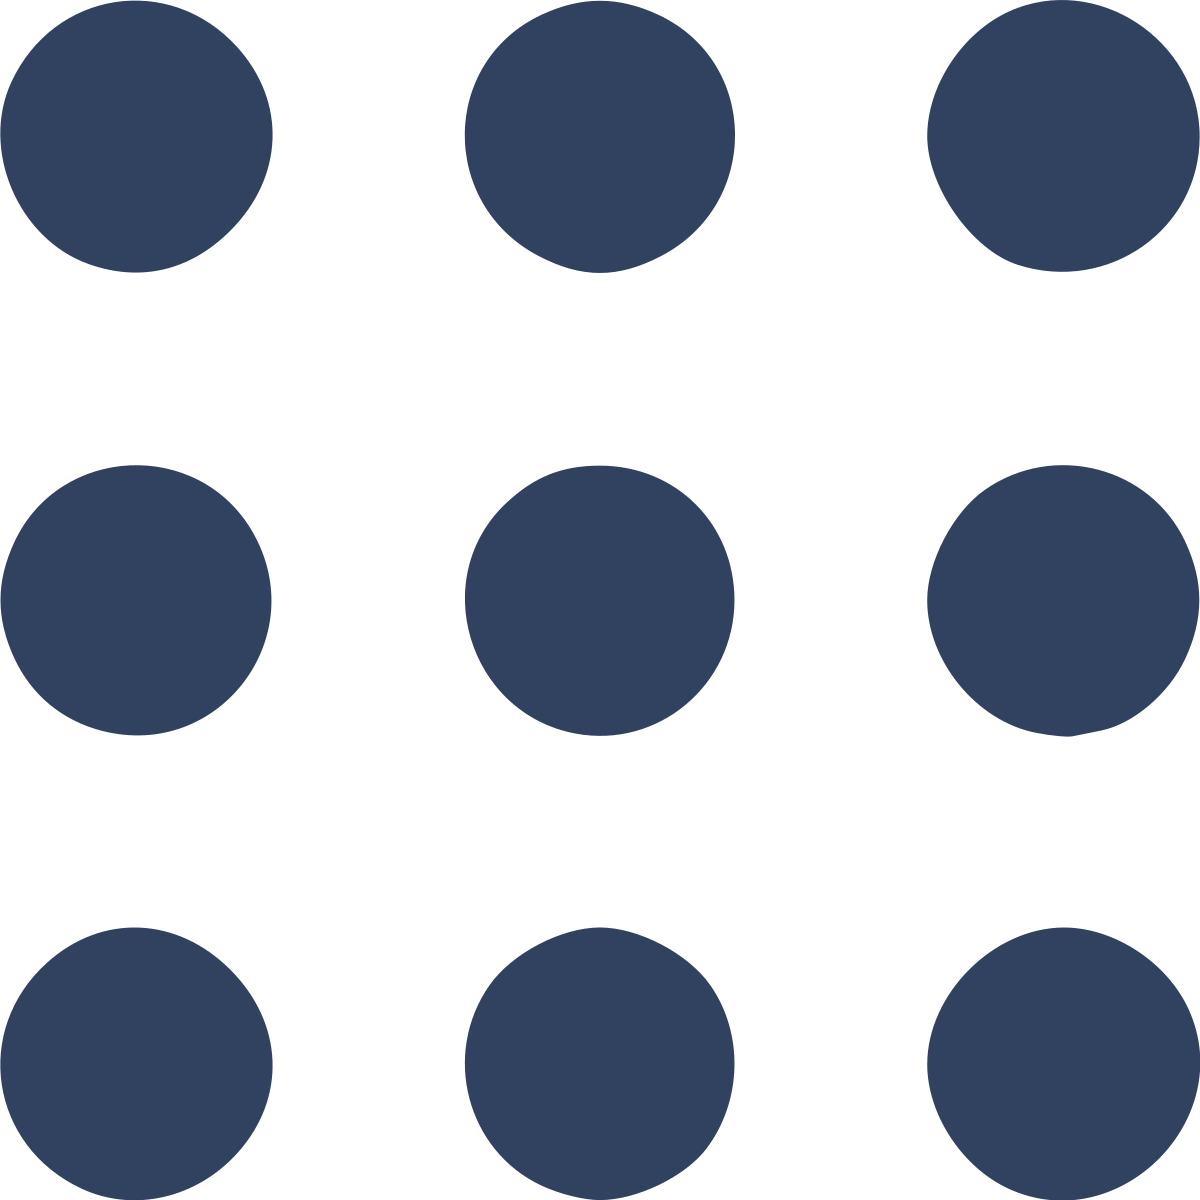
\includegraphics[height=0.75cm]{assets/ros.png}
  };
  \distrros{kinetic}{2016}
  \distrros{lunar}{2017}
  \distrros{melodic}{2018}
  \distrros{noetic}{2020}
  \draw[timeline, ROSBlue] (kinetic) -- (lunar);
  \draw[timeline, ROSBlue] (lunar) -- (melodic);
  \draw[timeline, ROSBlue] (melodic) -- (noetic);

  \node[inner sep=0pt] (ros2) at (\xLogo,\yRosTwo) {
    
\includegraphics[width=0.75cm]{assets/ros2.png}
  };

  \distrrostwo{foxy}{2020}
  \distrrostwo{galactic}{2021}
  \distrrostwo{humble}{2022}
  \distrrostwo{iron}{2023}
  \distrrostwo{jazzy}{2024}
  \distrrostwo{kilted}{2025}
  \distrrostwo{lyrical}{2026}
  \draw[timeline, ROSBlue] (foxy) -- (galactic);
  \draw[timeline, ROSBlue] (galactic) -- (humble);
  \draw[timeline, ROSBlue] (humble) -- (iron);
  \draw[timeline, ROSBlue] (iron) -- (jazzy);
  \draw[timeline, ROSBlue] (jazzy) -- (kilted);
  \draw[timeline, ROSBlue] (kilted) -- (lyrical);

  \begin{scope}[opacity=0.75]
    \def\eloquentYear{2019}
    \pgfmathsetmacro\x{2*(\eloquentYear-2016)};
    \node[event=1.5pt, fill=ROSBlue] (eloquent) at (\x,\yRosTwo){};
    \node[above=0.08 of eloquent,align=center, fill=white, inner sep=1pt]{\rosdistro{dashing}\\\rosdistro{eloquent}};
    \draw[timeline, ROSBlue] (eloquent) -- (foxy);
  \end{scope}

  \begin{scope}[opacity=0.75]
    \def\ardentYear{2018}
    \pgfmathsetmacro\x{2*(\ardentYear-2016)};
    \node[event=1.5pt, fill=ROSBlue] (ardent) at (\x,\yRosTwo){};
    \node[above=0.08 of ardent,align=center, fill=white, inner sep=1pt]{\rosdistro{ardent}-\\\rosdistro{crystal}};
    \draw[timeline, ROSBlue] (ardent) -- (eloquent);
  \end{scope}

  % Gazebo Classic
  \node[inner sep=0pt] (gazebo) at (\xLogo,\yGazebo) {
    
\includegraphics[width=0.75cm]{assets/Gazebo.png}
  };
  \gazeboversion{\textcolor{GazeboOrange}{7.x}}{2016}
  \gazeboversion{\textcolor{GazeboOrange}{9.x}}{2018}
  \gazeboversion{\textcolor{GazeboOrange}{11.x}}{2020}
  \gazeboversion{}{2023}
  \draw[timeline, GazeboOrange] (Gazebo2016) -- (Gazebo2018);
  \draw[timeline, GazeboOrange] (Gazebo2018) -- (Gazebo2020);
  \draw[timeline, GazeboOrange] (Gazebo2020) -- (Gazebo2023);

  % Ignition / Gazebo
  \node[inner sep=0pt] (ignition) at (\xLogo,\yIgnition) {
    
\includegraphics[width=0.75cm]{assets/Ignition.png}
  };
  \ignitionversion{\textcolor{IgnitionDarkOrange}{citadel}}{2020}
  \ignitionversion{\textcolor{IgnitionDarkOrange}{edifice}}{2021}
  \ignitionversion{\textcolor{IgnitionDarkOrange}{fortress}}{2022}
  \ignitionversion{\textcolor{IgnitionDarkOrange}{harmonic}}{2024}
  \ignitionversion{\textcolor{IgnitionDarkOrange}{ionic}}{2025}
  \ignitionversion{\textcolor{IgnitionDarkOrange}{jetty}}{2026}
  \draw[timeline, IgnitionLightOrange] (Ignition2020) -- (Ignition2021);
  \draw[timeline, IgnitionLightOrange] (Ignition2021) -- (Ignition2022);
  \draw[timeline, IgnitionLightOrange] (Ignition2022) -- (Ignition2024);
  \draw[timeline, IgnitionLightOrange] (Ignition2024) -- (Ignition2025);
  \draw[timeline, IgnitionLightOrange] (Ignition2025) -- (Ignition2026);

\end{tikzpicture}

\end{document}
